\mbox{}\\
\vspace{8cm}

This chapter is a reproduction of the following publication:

C. I. Mendes, E. Lizarazo, M. P. Machado, D. N. Silva, A. Tami, M. Ramirez, N. Couto, J. W. A. Rossen, J. A. Carriço, DEN-IM: dengue virus genotyping from amplicon and shotgun metagenomic sequencing. Microbial Genomics, Volume 6, Issue 3, March 2020. DOI: \url{https://doi.org/10.1099/mgen.0.000328}

The supplementary information referred throughout the text can be consulted in this chapter before the section of references. 

\ac{DENV} represents a public health threat and economic burden in affected countries. The risk of exposure to \ac{DENV} is increasing, not only because of travel to endemic regions, but also due to the broader dissemination of the mosquito vector, making the burden of dengue very significant. 

The availability of genomic data is key to understanding viral evolution and dynamics, supporting improved control strategies. Currently, the use of second-generation sequencing technologies, which can be applied both directly to patient samples (shotgun metagenomics) and to PCR-amplified viral sequences (amplicon sequencing), is the most informative approach to monitor viral dissemination and genetic diversity by providing, in a single methodological step, identification and characterization of the whole viral genome at the nucleotide level. This makes \ac{DENV} identification and characterization through genomic analysis by developing a software where the lessons learned in Chapters \ref{ch:paper1} and \ref{ch:paper2} are applied.

We have developed DEN-IM, a one-stop, user-friendly, containerised and reproducible workflow for the analysis of Dengue virus short-read sequencing data from both amplicon and shotgun metagenomics approaches. EN-IM was designed to perform a comprehensive analysis in order to generate either assemblies or consensus of full DENV coding sequences and to identify their serotype and genotype. DEN-IM can also detect all four DENV serotypes and the respective genotypes present in a spiked sample, raising the possibility that DEN-IM can play a role in the identification of co-infection cases whose prevalence is increasingly perceived in highly endemic areas. 

My contribution to this publication included the design, implementation and optimisation of the DEN-IM the workflow, including the creation of  the Docker containers for all dependencies. Two databases, one comprising 3830 \ac{DENV} sequences for the retrieval of the reads of interest from the input samples, and a second comprising of 161 sequences representing the genetic diversity of all \ac{DENV} sero and genotypes were constructed by me.  Additionally, I've also wrote the manuscript.


\cleardoublepage 

\begin{center}
\large
\textbf{DEN-IM: dengue virus genotyping from amplicon and shotgun metagenomic sequencing}
\end{center}

Catarina I Mendes$^1,2,*$, 
Erley Lizarazo$^2,*$,
Miguel P Machado$^1$, 
Diogo N Silva$^1$,
Adiana Tami$^2$,
Mário Ramirez$^1$, 
Natacha Couto$^2$, 
John W A Rossen$^2$ and João A Carriço$^1$


$^1$Instituto de Microbiologia, Instituto de Medicina Molecular, Faculdade de Medicina, Universidade de Lisboa, Lisboa, Portugal 

$^2$University of Groningen, University Medical Center Groningen, Department of Medical Microbiology and Infection Prevention, Groningen, The Netherlands

$^*$Contributed equally

\section{Abstract}

Dengue virus (DENV) represents a public health and economic burden in affected countries. The availability of genomic data is key to understanding viral evolution and dynamics, supporting improved control strategies. Currently, the use of High Throughput Sequencing (HTS) technologies, which can be applied both directly to patient samples (shotgun metagenomics) and PCR amplified viral sequences (targeted metagenomics), is the most informative approach to monitor the viral dissemination and genetic diversity.

Despite many advantages, these technologies require bioinformatics expertise and appropriate infrastructure for the analysis and interpretation of the resulting data. In addition, the many software solutions available can hamper reproducibility and comparison of results.
Here we present DEN-IM, a one-stop, user-friendly, containerised and reproducible workflow for the analysis of DENV sequencing data, both from shotgun and targeted metagenomics approaches. It is able to infer the DENV coding sequence (CDS), identify the serotype and genotype, and generate a phylogenetic tree. It can easily be run on any UNIX-like system, from local machines to high-performance computing clusters, performing a comprehensive analysis without the requirement of extensive bioinformatics expertise.

Using DEN-IM, we successfully analysed two DENV datasets. The first comprised 25 shotgun metagenomic sequencing samples of variable serotype and genotype, including an in vitro spiked sample containing the four known serotypes. The second dataset consisted of 106 targeted metagenomic sequences of DENV 3 genotype III where DEN-IM allowed detection of the intra-genotype diversity.
The DEN-IM workflow, parameters and execution configuration files, and documentation are freely available at \url{https://github.com/B-UMMI/DEN-IM}.

\subsection{Keywords}
dengue virus, surveillance, metagenomics, reproducibility, workflow, containerization, scalability
 
\section{Author Notes}
All supporting data, code and protocols have been provided within the article or through supplementary data files.

Metagenomic sequencing data available under BioProject PRJNA474413. DEN-IM reports for the analysed datasets are available in Figshare under https://doi.org/10.6084/m9.figshare.11316599.v1. Phylogeny inference trees for the dengue virus typing database available in Figshare at https://doi.org/10.6084/m9.figshare.11316599.v1. The supplemental material is available in Figshare at https://doi.org/10.6084/m9.figshare.11316599.v1. DEN-IM’s source code and documentation available at https://github.com/B-UMMI/DEN-IM.

\section{Abbreviations}
 
\ac{CDS}; 
Dengue virus ( \ac{DENV}); 
\ac{HPC}; 
\ac{HTS}; 
\ac{NCR}; 
\ac{QC}; 
Reverse Transcription Polymerase Chain Reaction (\ac{RT-PCR})

\section{Data Summary}

\begin{enumerate}
    \item The supplemental material and tables are available at Figshare under https://doi.org/10.6084/m9.figshare.9963812
    \item The 106 DENV-3 targeted metagenomics paired-end short-read datasets are available under BioProject PRJNA394021. The 25 shotgun metagenomics dataset is available under BioProject PRJNA474413. The accession number for all the samples in the shotgun metagenomics dataset are available in the Supplementary material
    \item The accession numbers for the 41 samples, belonging to zika virus, chikungunya virus and yellow fever virus shotgun and targeted metagenomic datasets are available in the Supplementary material. 
    \item DEN-IM reports for the analysed datasets are available at Figshare  (https://doi.org/10.6084/m9.figshare.9318851).
    \item Phylogeny inference trees for the dengue virus typing database available at Figshare (https://doi.org/10.6084/m9.figshare.9331826).
    \item Code for the DEN-IM workflow is available at \url{https://github.com/B-UMMI/DEN-IM} and documentation, including step-by-step tutorials, is available at \url{https://github.com/B-UMMI/DEN-IM/wiki}.
\end{enumerate}

\section{Impact Statement}
The risk of exposure to DENV is increasing not only by travelling to endemic regions, but also due to the broader dissemination of the mosquito, making the burden of dengue very significant.

The decreasing costs and wider availability of HTS makes it an ideal technology to monitor DENV’s transmission. Metagenomics approaches decrease the time to obtain nearly complete DENV sequences without the need for time-consuming viral culture through the direct processing and sequencing of patient samples. A ready to use bioinformatics workflow, enabling the reproducible analysis of DENV, is therefore particularly relevant for the development of a straightforward HTS workflow.

DEN-IM was designed to perform a comprehensive analysis in order to generate either assemblies or consensus of full DENV CDSs and to identify their serotype and genotype. DEN-IM can also detect all four DENV genotypes present in a spiked sample, raising the possibility that DEN-IM can play a role in the identification of co-infection cases whose prevalence is increasingly appreciated in highly endemic areas. Although being ready-to-use, the DEN-IM workflow can be easily customised to the user’s needs.

DEN-IM enables reproducible and collaborative research, being accessible to a wide group of researchers regardless of their computational expertise and resources available.

\section{Introduction}

The Dengue virus (DENV), a single-stranded positive-sense RNA virus belonging to the Flavivirus genus, is one of the most prevalent arboviruses and is mainly concentrated in tropical and subtropical regions. Infection with DENV results in symptoms ranging from mild fever to haemorrhagic fever and shock syndrome \citep{organization_dengue_2009}. Transmission to humans occurs through the bite of Aedes mosquitoes, namely Aedes aegypti and Aedes albopictus \citep{diamond_molecular_2015}. In 2010, it was predicted that the burden of dengue disease reached 390 million cases/year worldwide \citep{bhatt_global_2013}. The high morbidity and mortality of dengue makes it the arbovirus with the highest clinical significance \citep{lourenco_challenges_2018}. DENV is a significant public health challenge in countries where the infection is endemic due to the high health and economic burden. Despite the emergence of novel therapies and ecological strategies to control the mosquito vector, there are still important knowledge gaps in the virus biology and its epidemiology \citep{diamond_molecular_2015}.

The viral genome of $\sim$11,000 nucleotides, consists of a CDS of approximately 10.2 Kb that is translated into a single polyprotein encoding three structural proteins (capsid - C, premembrane - prM, envelope - E) and seven non-structural proteins (NS1, NS2A, NS2B, NS3, NS4A, NS4B and NS5). Additionally, the genome contains two Non-Coding Regions (NCRs) at their 5’ and 3’ ends \citep{leitmeyer_dengue_1999}.

DENV can be classified into four serotypes (1, 2, 3 and 4), differing from each other from 25\% to 40\% at the amino acid level. They are further classified into genotypes that vary by up to 3\% at the amino acid level \citep{diamond_molecular_2015}. The DENV-1 serotype comprises five genotypes (I-V), DENV-2 groups six (I-VI, also named American, Cosmopolitan, Asian-American, Asian II, Asian I and Sylvatic), DENV-3 four (I-III and V), and DENV-4 also four (I-IV).

Although real-time reverse transcription polymerase chain reaction (RT-PCR) will probably remain the front line in Dengue etiological diagnosis, the implementation of a surveillance system relying on HTS technologies allows the simultaneous identification and characterization by serotyping and genotyping of DENV cases at the nucleotide level in a single methodological step. Due to the high sensitivity of these technologies, previous studies showed that viral sequences can be directly obtained from patient sera using a shotgun metagenomics approach \citep{yozwiak_virus_2012}. Alternatively, HTS can be used in a targeted metagenomics approach in which a PCR step is used to pre-amplify viral sequences before sequencing. In recent years, HTS has been successfully used as a tool for identification of DENV directly from clinical samples \citep{yozwiak_virus_2012, lee_clinical_2017}. This also allows the rapid identification of the serotype and genotype important for disease management as the genotype may be associated with disease outcome \citep{fatima_serotype_2011}.

Several initiatives aim to facilitate the identification of the DENV serotype and genotype from HTS data. The Genome Detective project (https://www.genomedetective.com/) offers an online Dengue Typing Tool (https://www.genomedetective.com/app/typingtool/dengue/) \citep{fonseca_computational_2019} relying on BLAST and phylogenetic methods in order to identify the closest serotype and genotype, but it requires as input assembled genomes in FASTA format. The same project also offers the Genome Detective Typing Tool (https://www.genomedetective.com/app/typingtool/virus/) \citep{vilsker_genome_2019} identifying viruses present in a sample. Additionally, there are several tools available for viral read identification and assembly, such as VIP \citep{li_vip_2016}, virusTAP \citep{yamashita_virustap_2016} and drVM \citep{lin_drvm_2017}, but none performs genotyping of the identified reads.

We developed DEN-IM as a ready-to-use, one-stop, reproducible bioinformatic analysis workflow for the processing and phylogenetic analysis of DENV using paired-end raw HTS data. DEN-IM is implemented in Nextflow \citep{di_tommaso_nextflow_2017}, a workflow manager software that uses Docker (https://www.docker.com) containers with pre-installed software for all the workflow tools. The DEN-IM workflow, as well as parameters and documentation, are available at \url{https://github.com/B-UMMI/DEN-IM}.

\section{The DEN-IM Workflow}

DEN-IM is a user-friendly automated workflow enabling the analysis of shotgun or targeted metagenomics data for the identification, serotyping, genotyping, and phylogenetic analysis of DENV, as represented in Figure \ref{fig:chap4_figure1}, accepting as input raw paired-end sequencing data (FASTQ files) and informing the user with an interactive and comprehensive HTML report (Supplementary Figure ), as well as providing output files of the whole pipeline. 

\begin{figure*}[h!]
\centering
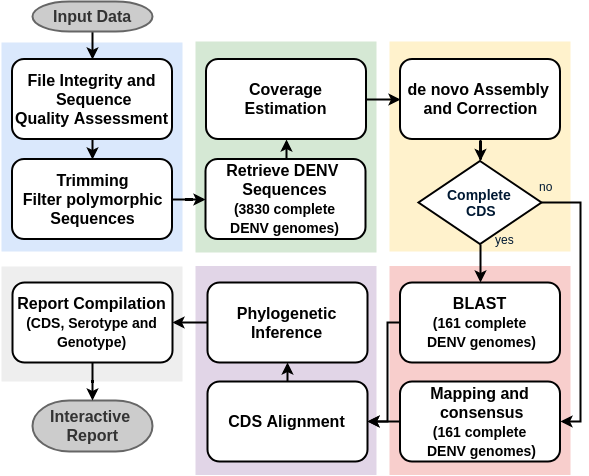
\includegraphics[width=\textwidth]{figures/chapter 4/Figure1_DEN-IM_Diagram.png}
\caption{The DEN-IM workflow separated into five different components. The raw sequencing reads are provided as input to the first block (in blue), responsible for quality control and elimination of low-quality reads and sequences. After successful preprocessing of the reads, these enter the second block (green) for retrieval of the DENV reads using the mapping database of 3858 complete DENV genomes as a reference. This block also provides an initial estimate of the sequencing depth. After the de novo assembly and assembly correction block (yellow), the CDSs are retrieved and then classified with the reduced-complexity DENV typing database containing 161 sequences representing the known diversity of DENV serotypes and genotypes (red). If a complete CDS fails to be assembled, the reads are mapped against the DENV typing database and a consensus sequence is obtained for classification and phylogenetic inference. All CDSs are aligned and compared in a phylogenetic analysis (purple). Lastly, a report is compiled (grey) with the results of all the blocks of the workflow.}
\label{fig:chap4_figure1}
\end{figure*}

It is implemented in Nextflow, a workflow management system that allows the effortless deployment and execution of complex distributed computational workflows in any UNIX-based system, from local machines to \ac{HPC} with a container engine installation, such as Docker (https://www.docker.com/), Shifter \citep{gerhardt_shifter_2017} or Singularity \citep{kurtzer_singularity_2017}. DEN-IM integrates Docker containerised images, compatible with other container engines, for all the tools necessary for its execution, ensuring reproducibility and the tracking of both software code and version, regardless of the operating system used. 

Users can customise the workflow execution either by using command line options or by modifying the simple plain-text configuration files. To make the execution of the workflow as simple as possible, a set of default parameters and directives is provided. An exhaustive description of each parameter is available as Supplementary material (see \ref{}).

The local installation of the DEN-IM workflow, including the docker containers with all the tools needed and the curated DENV database, requires 15 Gigabytes (Gb) of free disk space. The minimum requirements to execute the workflow are at least 5 Gb of memory and 4 CPUs. The disk space required for execution depends greatly on the size of the input data, but for the datasets used in this article, DEN-IM generates approximately 5 Gb of data per Gb input data.
DEN-IM workflow can be divided into the following components:

\subsubsection{Quality Control and Trimming}

The Quality Control (QC) and Trimming block starts with a process to verify the integrity of the input data. If the sequencing files are corrupted, the execution of the analysis of that sample is terminated. The sequences are then processed by FastQC (https://www.bioinformatics.babraham.ac.uk/projects/fastqc/, version 0.11.7) to determine the quality of the individual base pairs of the raw data files. The low-quality bases and adapter sequences are trimmed by Trimmomatic \citep{schmieder_quality_2011} (version 0.36). In addition, paired-end reads with a read length shorter than 55 nucleotides after trimming are removed from further analyses. Lastly, the low complexity sequences, containing over 50\% of poly-A, poly-N or poly-T nucleotides, are filtered out of the raw data using PrinSeq \citep{schmieder_quality_2011} (version 0.10.4).

\subsubsection{Retrieval of DENV sequences}

In the second step, DENV sequences are selected from the sample using Bowtie2 \citep{langmead_fast_2012} (version 2.2.9) and Samtools \citep{langmead_fast_2012} (version 1.4.1). As a reference we provide the DENV mapping database, a curated DENV database composed of 3830 complete DENV genomes. An in-depth description of this database is available as Supplementary material (see \ref{}). A permissive approach is followed by allowing for mates to be kept in the sample even when only one read maps to the database in order to keep as many DENV derived reads as possible. The output of this block is a set of processed reads of putative DENV origin.

\subsubsection{Assembly}

DEN-IM applies a two-assembler approach to generate assemblies of the DENV CDS. To obtain a high confidence assembly, the processed reads are first de novo assembled with SPAdes \citep{bankevich_spades_2012} (version 3.12.0). If the full CDS fails to be assembled into a single contig, the data is re-assembled with the MEGAHIT assembler \citep{li_megahit_2015} (version 1.1.3), a more permissive assembler developed to retrieve longer sequences from metagenomics data. The resulting assemblies are corrected with Pilon \citep{walker_pilon_2014} (version 1.22) after mapping the processed reads to the assemblies with Bowtie2.

If more than one complete CDS is present in a sample, each of the sequences will follow the rest of the DEN-IM workflow independently. If no full CDS is assembled neither with SPAdes nor with MEGAHIT, the processed reads are passed on to the next module for consensus generation by mapping, effectively constituting DEN-IM’s two-pronged approach using both assemblers and mapping.

\subsubsection{Typing}

For each DENV complete CDS, the serotype and genotype is determined with the Seq\_Typing tool (\url{https://github.com/B-UMMI/seq\_typing}, version 2.0) \citep{machado_epidemiological_2017} using BLAST \citep{altschul_gapped_1997} and the custom Typing database of DENV containing 161 complete sequences (see \ref{}). The tool determines which reference sequence is more closely related to the query based on the identity and length of the sequence covered, returning the serotype and genotype of the reference sequence

If a complete CDS fails to be obtained through the assembly process, the processed reads are mapped against the same DENV typing database, with Bowtie2, using the Seq\_Typing tool, with similar criteria for coverage and identity to those used with the BLAST approach. If a type is determined, the consensus sequence obtained follows through to the next step in the workflow. Otherwise, the sample is classified as Non-Typable and its process terminated.

\subsubsection{Phylogeny}

All DENV complete CDSs and consensus sequences analysed in a workflow execution are aligned with MAFFT \citep{nakamura_parallelization_2018} (version 7.402). By default, or if the number of samples analysed is less than 4, four representative sequences for each DENV serotype (1 to 4) from NCBI are also included in the alignment. The NCBI references included are NC\_001477.1 (DENV-1), NC\_001474.2 (DENV-2), NC\_001475.2 (DENV-3) and NC\_002640.1 (DENV-4). The closest reference sequence to each analysed sample in the DENV typing database to each analysed sample can also be retrieved and included in the alignment. With the resulting alignment, a Maximum Likelihood tree is constructed with RaXML \citep{stamatakis_raxml_2014} (version 8.2.11). 

\subsubsection{Output and Report}

The output files of all tools in DEN-IM’s workflow are stored in the ’results’ folder in the directory of DEN-IM’s execution, as well as the execution log file DEN-IM and for each component. 

The HTML report (Supplementary Figure \ref{}), stored in the ’pipeline\_results’ directory contains all results divided into four sections: report overview, tables, charts and phylogenetic tree. The report overview and all tables allow for selection, filtering and highlighting of particular samples in the analysis. All tables have information on if a sample failed or passed the quality control metrics highlighted by green, yellow or red signs for pass, warning and fail messages, respectively. 

The \textit{in silico} typing table contains the results of the serotype and genotype of each CDS analysed, as well as identity, coverage and GenBank ID of the closest reference in the DENV typing database. The quality control table shows information regarding the number of raw base pairs and number of reads in the raw input files and the percentage of trimmed reads. The mapping table includes the results for the mapping of the trimmed reads to the DENV mapping database, including the overall alignment rate, and an estimation of the sequence depth including only the DENV reads. For the assembly statistics table, the number of CDSs in each sample, the number of contigs and the number of assembled base pairs generated by either SPAdes or MEGAHIT assemblers is included. The number of contigs and assembled base pairs after correction with Pilon is also presented in the table. The assembled contig size distribution scatter plot is available in the chart section, showing the contig size distribution for the Pilon corrected assembled CDSs.

Lastly, a phylogenetic tree is included, rooted at midpoint for visualisation purposes, and with each tip coloured according to the genotyping results. If the option to retrieve the closest typing reference is selected, these sequences are also included in the tree with respective typing metadata. The tree can be displayed in several conformations provided by Phylocanvas JavaScript library (\url{http://phylocanvas.net}, version 2.8.1) and it is possible to zoom in or collapse selected branches. The support bootstrap values of the branches can be displayed, and the tree can be exported as a Newick tree file or as a PNG image.

\section{Software comparison}

DEN-IM offers a core assembly functionality, leveraging a de novo and consensus assembly approach, to obtain a full CDS sequence to perform geno- and serotyping, followed by phylogenetic positioning of the samples analysed. This results in a phylogenetic tree showing the genotyping results, presented in an HTML file.

There are several alternative tools, both command line and online based, capable of identifying DENV reads and performing assembly (Table \ref{tab:ch4_table1}). VIP and drVM are both stand-alone pipelines, like DEN-IM, and several components overlap with DEN-IM’s but the retrieval of viral sequences is not targeted for DENV, and no serotyping and genotyping is performed. VIP performs a phylogenetic analysis against the reference database. VirusTAP is a web server for the identification of viral reads using the ViPR and IRD databases, or alternatively with the RefSeq Virus database. GenomeDetective is also a web service that provides two tools, one for the assembly of viral sequences from raw data (Virus tool) and another for serotyping and genotyping of DENV fasta sequences (Dengue Typing tool). Both tools need to be run consecutively, with the Virus Tool providing a link to redirect to the Dengue Typing tool when a DENV sequence is identified.


\begin{table}[h!]
\caption{DEN-IM’s workflow comparison with different tools for the identification and genotyping of DENV from sequencing data.}
\label{tab:ch4_table1}
\resizebox{\textwidth}{!}{%
\begin{tabular}{@{}lcccccc@{}}
\toprule
\textbf{Tool} &
  \textbf{Quality Control} &
  \textbf{DENV Sequence Retrieval} &
  \textbf{Assembly} &
  \textbf{Typing} &
  \textbf{Phylogeny} &
  \textbf{Report} \\ \midrule
DEN-IM &
  \checkmark &
  \checkmark &
  \checkmark &
  \checkmark &
  \checkmark &
  \begin{tabular}[c]{@{}c@{}}\checkmark (one report \\ with all samples \\ analysed)\end{tabular} \\
VIP &
  \checkmark &
  \checkmark$^1$ &
  \checkmark &
  X &
  \checkmark &
  \checkmark \\
VirusTAP &
  \checkmark &
  \checkmark$^1$ &
  \checkmark &
  X &
  X &
  \begin{tabular}[c]{@{}c@{}}\checkmark (web-based, \\ one per sample, \\ downloadable)\end{tabular} \\
drVM &
  \checkmark &
  \checkmark$^1$ &
  \checkmark &
  X &
  X &
  X \\
\begin{tabular}[c]{@{}l@{}}GenomeDetective \\ Virus Tool\end{tabular} &
  \checkmark &
  X &
  \checkmark &
  X &
  X &
  \begin{tabular}[c]{@{}c@{}}\checkmark (web-based, \\ one per sample)\end{tabular} \\
\begin{tabular}[c]{@{}l@{}}GenomeDetective \\ Dengue Typing Tool\end{tabular} &
  X &
  X &
  X &
  \checkmark$^2$ &
  X &
  \begin{tabular}[c]{@{}c@{}}\checkmark (web-based, \\ one per sample)\end{tabular} \\ \bottomrule
\end{tabular}%
}
\item $^1$ Targeted for viral sequences, but not specific for DENV
\item $^2$ Sequence file can be received from GenomeDetective Virus Tool, as well as independently uploaded
\end{table}

Of all the tools listed in Table \ref{tab:ch4_table1}, only Genome Detective offers a tool to determine the DENV sero- and genotype from a fasta sequence, but the need to run their virus identification tool prior to obtain a sequence from the raw sequencing data increases the time to obtain a typing result, especially when a large number of sequences needs to be analysed. Moreover, these tools are not open source, so we are unable to compare the methodology used with our own. Additionally, there might be privacy issues in submitting data to external services, like VirusTAP and GenomeDetective, especially when handling metagenomics data that contain human sequences subjected to strict privacy laws in most countries. Therefore, a stand-alone tool is preferable for these analyses since these can be run in secure local environments. DEN-IM’s main advantage when compared to web-based platforms is the ability to analyse batches of samples in a scalable manner, obtaining a report summarizing all the samples analysed and a phylogeny analysis of all DENV CDSs recovered.


\section{Results}

To evaluate the DEN-IM workflow performance, we analysed three datasets, one containing shotgun metagenomics sequencing data of patient samples (see Table \ref{}), a second with amplicon sequencing data, a set with 106 paired-end samples obtained from Parameswaran et al \citep{parameswaran_intrahost_2017} and another set with 78 single-end samples available under BioProject PRJNA321963, and a third dataset of publicly available sequences, both from amplicon and shotgun metagenomics, containing 45 chikungunya virus (CHIKV) samples, 66 zika virus (ZKV), and 21 yellow fever virus (YFV) samples (see Table \ref{}). All analyses were executed with the default resources and parameters (available at \url{https://github.com/B-UMMI/DEN-IM}). In the shotgun metagenomics and the single-end amplicon sequencing datasets the closest typing reference in the final tree and the NCBI DENV references for each serotype were included in the phylogenetic analysis. The resulting reports for each dataset are available on Figshare at \url{https://doi.org/10.6084/m9.figshare.9318851}.

\subsubsection{Shotgun metagenomics dataset}

We analysed a dataset containing 22 shotgun metagenomics paired-end short-read Illumina sequencing samples from positive dengue cases, one positive control (purified from a DENV culture), one negative control (blank), and an in vitro spiked sample containing the 4 DENV serotypes (see \ref{}). On average, each sample took 7 minutes to analyse. A total of 75 CPU hours were used to analyse the 25 samples, with a total of 17 Gb in size. This analysis resulted in 69 Gb of data. 
The negative control and the 92-1001 sample had no reads after trimming and filtering of low complexity reads, therefore they were removed from further analysis (see \ref{}). When mapping to the DENV mapping database, the percentage of DENV reads in the 21 clinical samples, positive control and spiked sample passing QC ranged from 0.01\% (sample UCUG0186) to 85.38\% (sample Positive Control - PC). After coverage depth estimation, the analysis of the samples 91-0115 and UCUG0186 was terminated due to a low proportion of DENV reads (0.05\% and 0.01\% respectively). Therefore, they failed to meet the threshold criterion of having an estimated depth of coverage of $\geq$10x (estimated coverages of 3.17x and 5.65x, respectively). Sequence data of sample 91-0106 contained only 960 DENV reads (0.03\%) but these were successfully assembled into a CDS with an estimated depth of coverage of 14.71x.

In the assembly module, the remaining 19 samples, the spiked sample and the PC were assembled with DEN-IM’s two assembler approach. Twenty-four full CDS were assembled (see \ref{}), even in samples originally having DENV read content as low as 0.03\% of the total reads. Sixteen samples, including the spiked sample and the positive control, were assembled in the first step with the SPAdes assembler, and five in the second with the MEGAHIT assembler. In the spiked sample, all four CDSs were successfully assembled and recovered.

Serotype and genotype were successfully determined for the 24 DENV CDSs by BLAST (see \ref{}). The most common were serotype 2 genotype III (Asian American) and serotype 4 genotype II, with 8 samples each (33\%), followed by serotype 3 genotype III (n=5, 21\%), serotype 1 genotype V (n=2, 8\%) and serotype 2 genotype V (Asian I) (n=1, 4\%). All CDSs recovered and the respective closest reference genome in the typing database were aligned and a maximum likelihood phylogenetic tree was obtained to visualise the relationship between the samples (Figure \ref{fig:chap4_figure2}). There was a perfect concordance between the results of serotyping and genotyping and the major groups in the tree.
Four distinct CDSs were assembled for the spiked sample that resulted in different coverages of each serotype CDS (2032x times coverage for DENV-2, 229x coverage for DENV-1, 76x coverage for DENV-3 and 30x times coverage for DENV-4), in accordance with the ranking order of the real-time RT-PCR results (see \ref{}).

\begin{figure*}[h!]
\centering
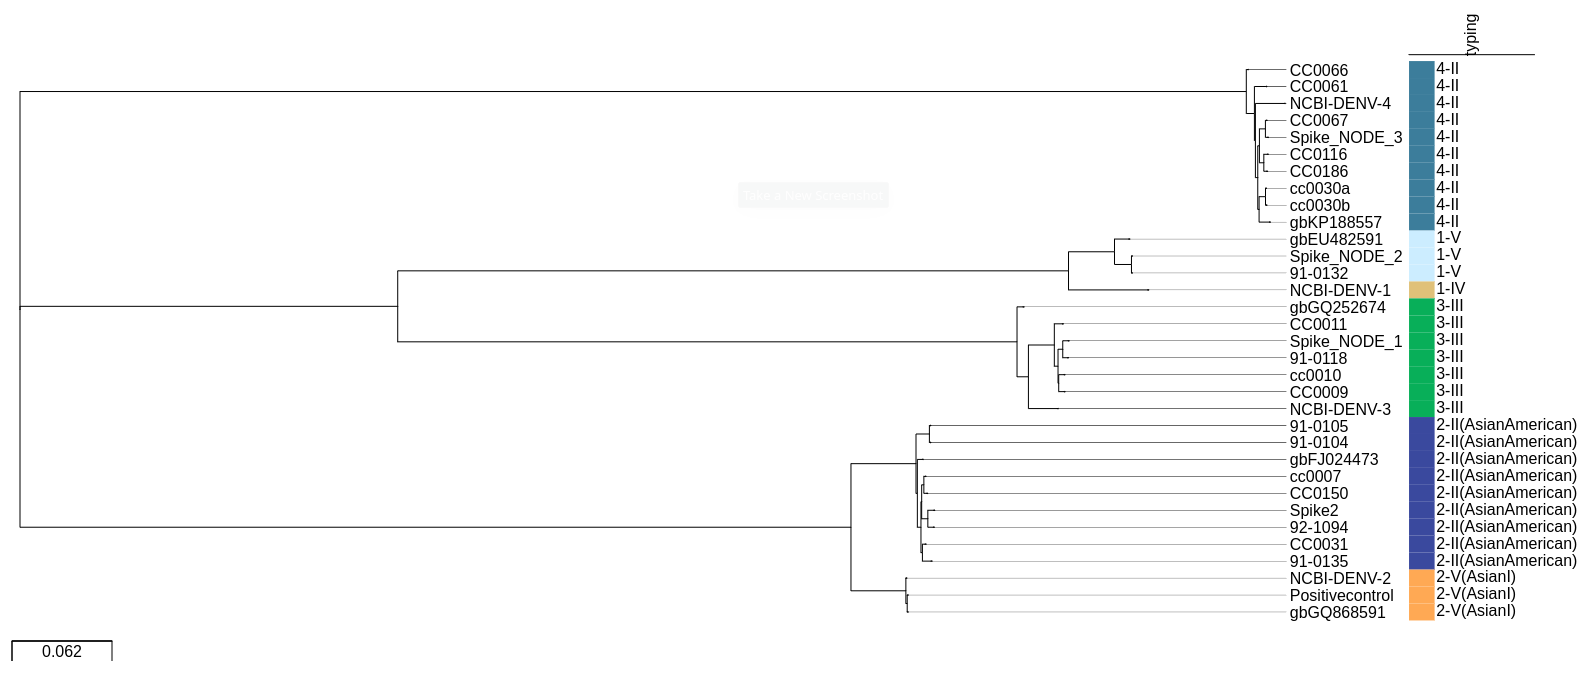
\includegraphics[width=\textwidth]{figures/chapter 4/Figure2_nobranchlabels.png}
\caption{Phylogenetic reconstruction of the shotgun metagenomic dataset. Maximum Likelihood tree in the DEN-IM report for the 24 complete CDSs (n=21 samples) obtained with the metagenomics dataset, the respective closest references in the typing database (identified by their GenBank ID), and the NCBI DENV references for each serotype (NCBI-DENV-1: NC\_001477.1, NCBI-DENV-2: NC\_001474.2, NCBI-DENV-3: NC\_001475.2, NCBI-DENV-4: NC\_002640.1). The tree is midpoint rooted for visualisation purposes and the scale represents average substitutions per site. The colours depict the DENV genotyping results.}
\label{fig:chap4_figure2}
\end{figure*}

\subsubsection{The Amplicon Sequencing Dataset}

To validate DEN-IM’s performance in a amplicon sequencing approach, a dataset of 106 paired-end HTS samples of PCR products using primers targeting DENV-3 (27) were analysed (see \ref{}). On average, each sample took 5 minutes to analyse. The 106 samples, with 51 Gb in size, took 3622 CPU hours to be analysed, resulting in 424 Gb of data. 

No samples failed the quality control block (see Table \ref{}). The proportion of DENV reads ranged from 24.72\% (SRR5821236) to 99.81\% (SRR5821254) of the total processed reads. The samples with less than 70\% DENV DNA were taxonomically profiled with Kraken2 (28) and the minikraken2\_v2 database (\url{ftp://ftp.ccb.jhu.edu/pub/data/kraken2_dbs/minikraken2_v2_8GB_201904_UPDATE.tgz}) and the source of contamination was determined to have come largely from Human DNA (see Table \ref{}).

Of the 106 samples, 43 (41\%) managed to assemble a complete CDS sequence (see Table \ref{}) whereas a mapping approach was used for the remaining 63 samples (60\%) and a consensus CDS was generated. For the assembled CDSs, all but one were assembled with MEGAHIT after not producing a full CDS with SPAdes. Moreover, pronounced variation on the size of the assembled contigs is evident in the contig size distribution plot (see \ref{}).

All 106 CDSs recovered belonged to serotype 3 genotype III. Despite the same classification, the maximum likelihood tree indicates that there is detectable genetic diversity within the dataset (486 SNPs in 10237 nucleotides) (Figure \ref{fig:chap4_figure3}).

\begin{figure*}[h!]
\centering
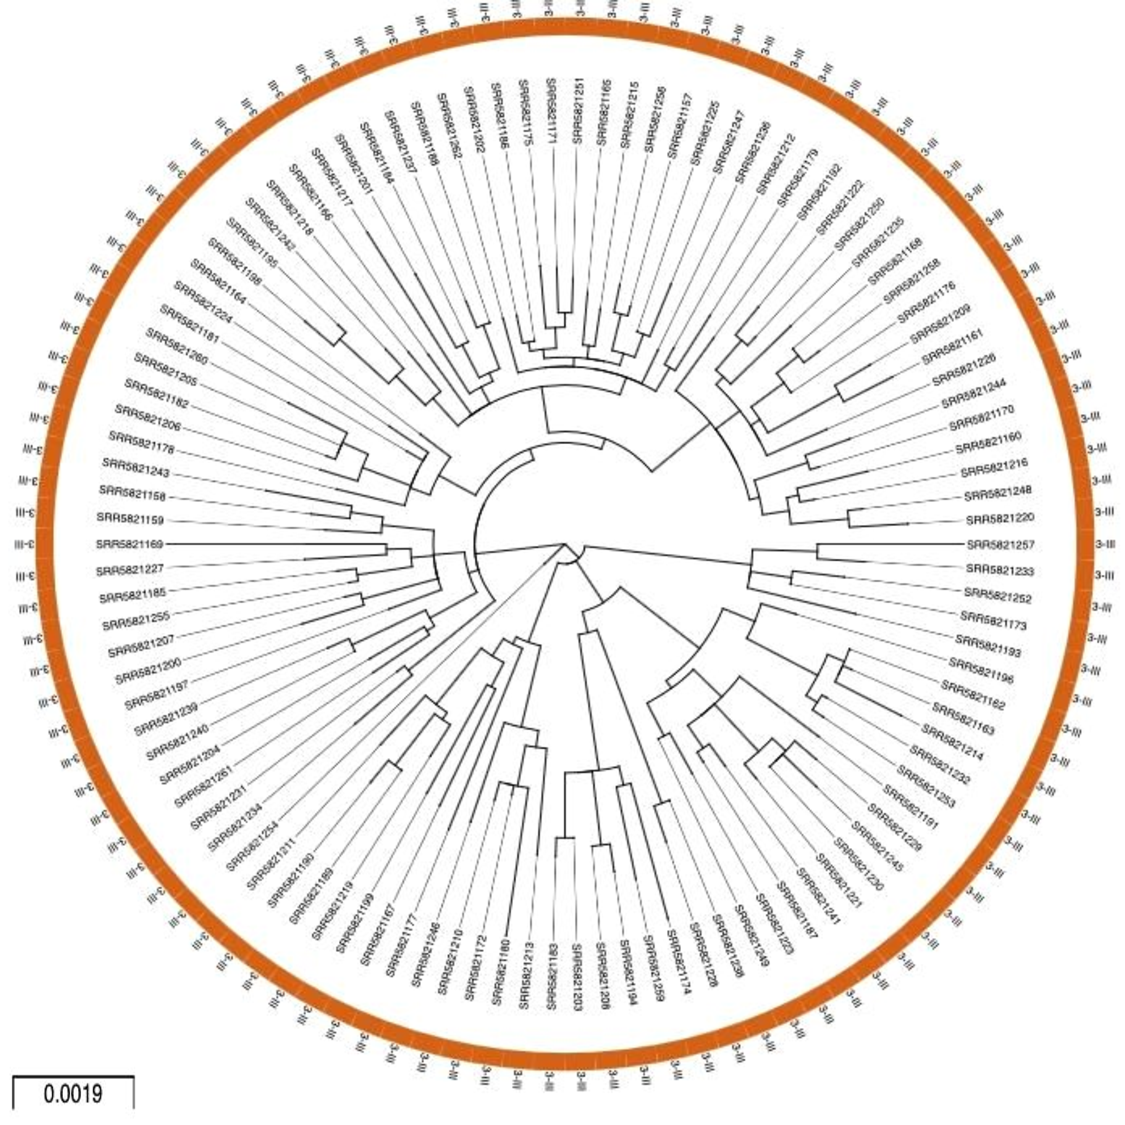
\includegraphics[width=\textwidth]{figures/chapter 4/Figure3_phylo_tree_amplicon.pdf}
\caption{Phylogenetic reconstruction of the paired-end targeted metagenomic dataset. Maximum likelihood circular tree in the DEN-IM report for the 106 complete CDSs obtained with the targeted metagenomics dataset (n=106). All samples belong to serotype 3 genotype III. The scale represents average substitutions per site.}
\label{fig:chap4_figure3}
\end{figure*}

A second amplicon dataset, containing 78 DENV-1 single-end samples recovered from different Aedes aegypti isofemale hosts were analysed (see \ref{}). On average, each sample took 3 minutes to analyse. The 78 samples, with 19 Gb in size, took 278 CPU hours to be analysed, resulting in 203 Gb of data.

\begin{figure*}[h!]
\centering
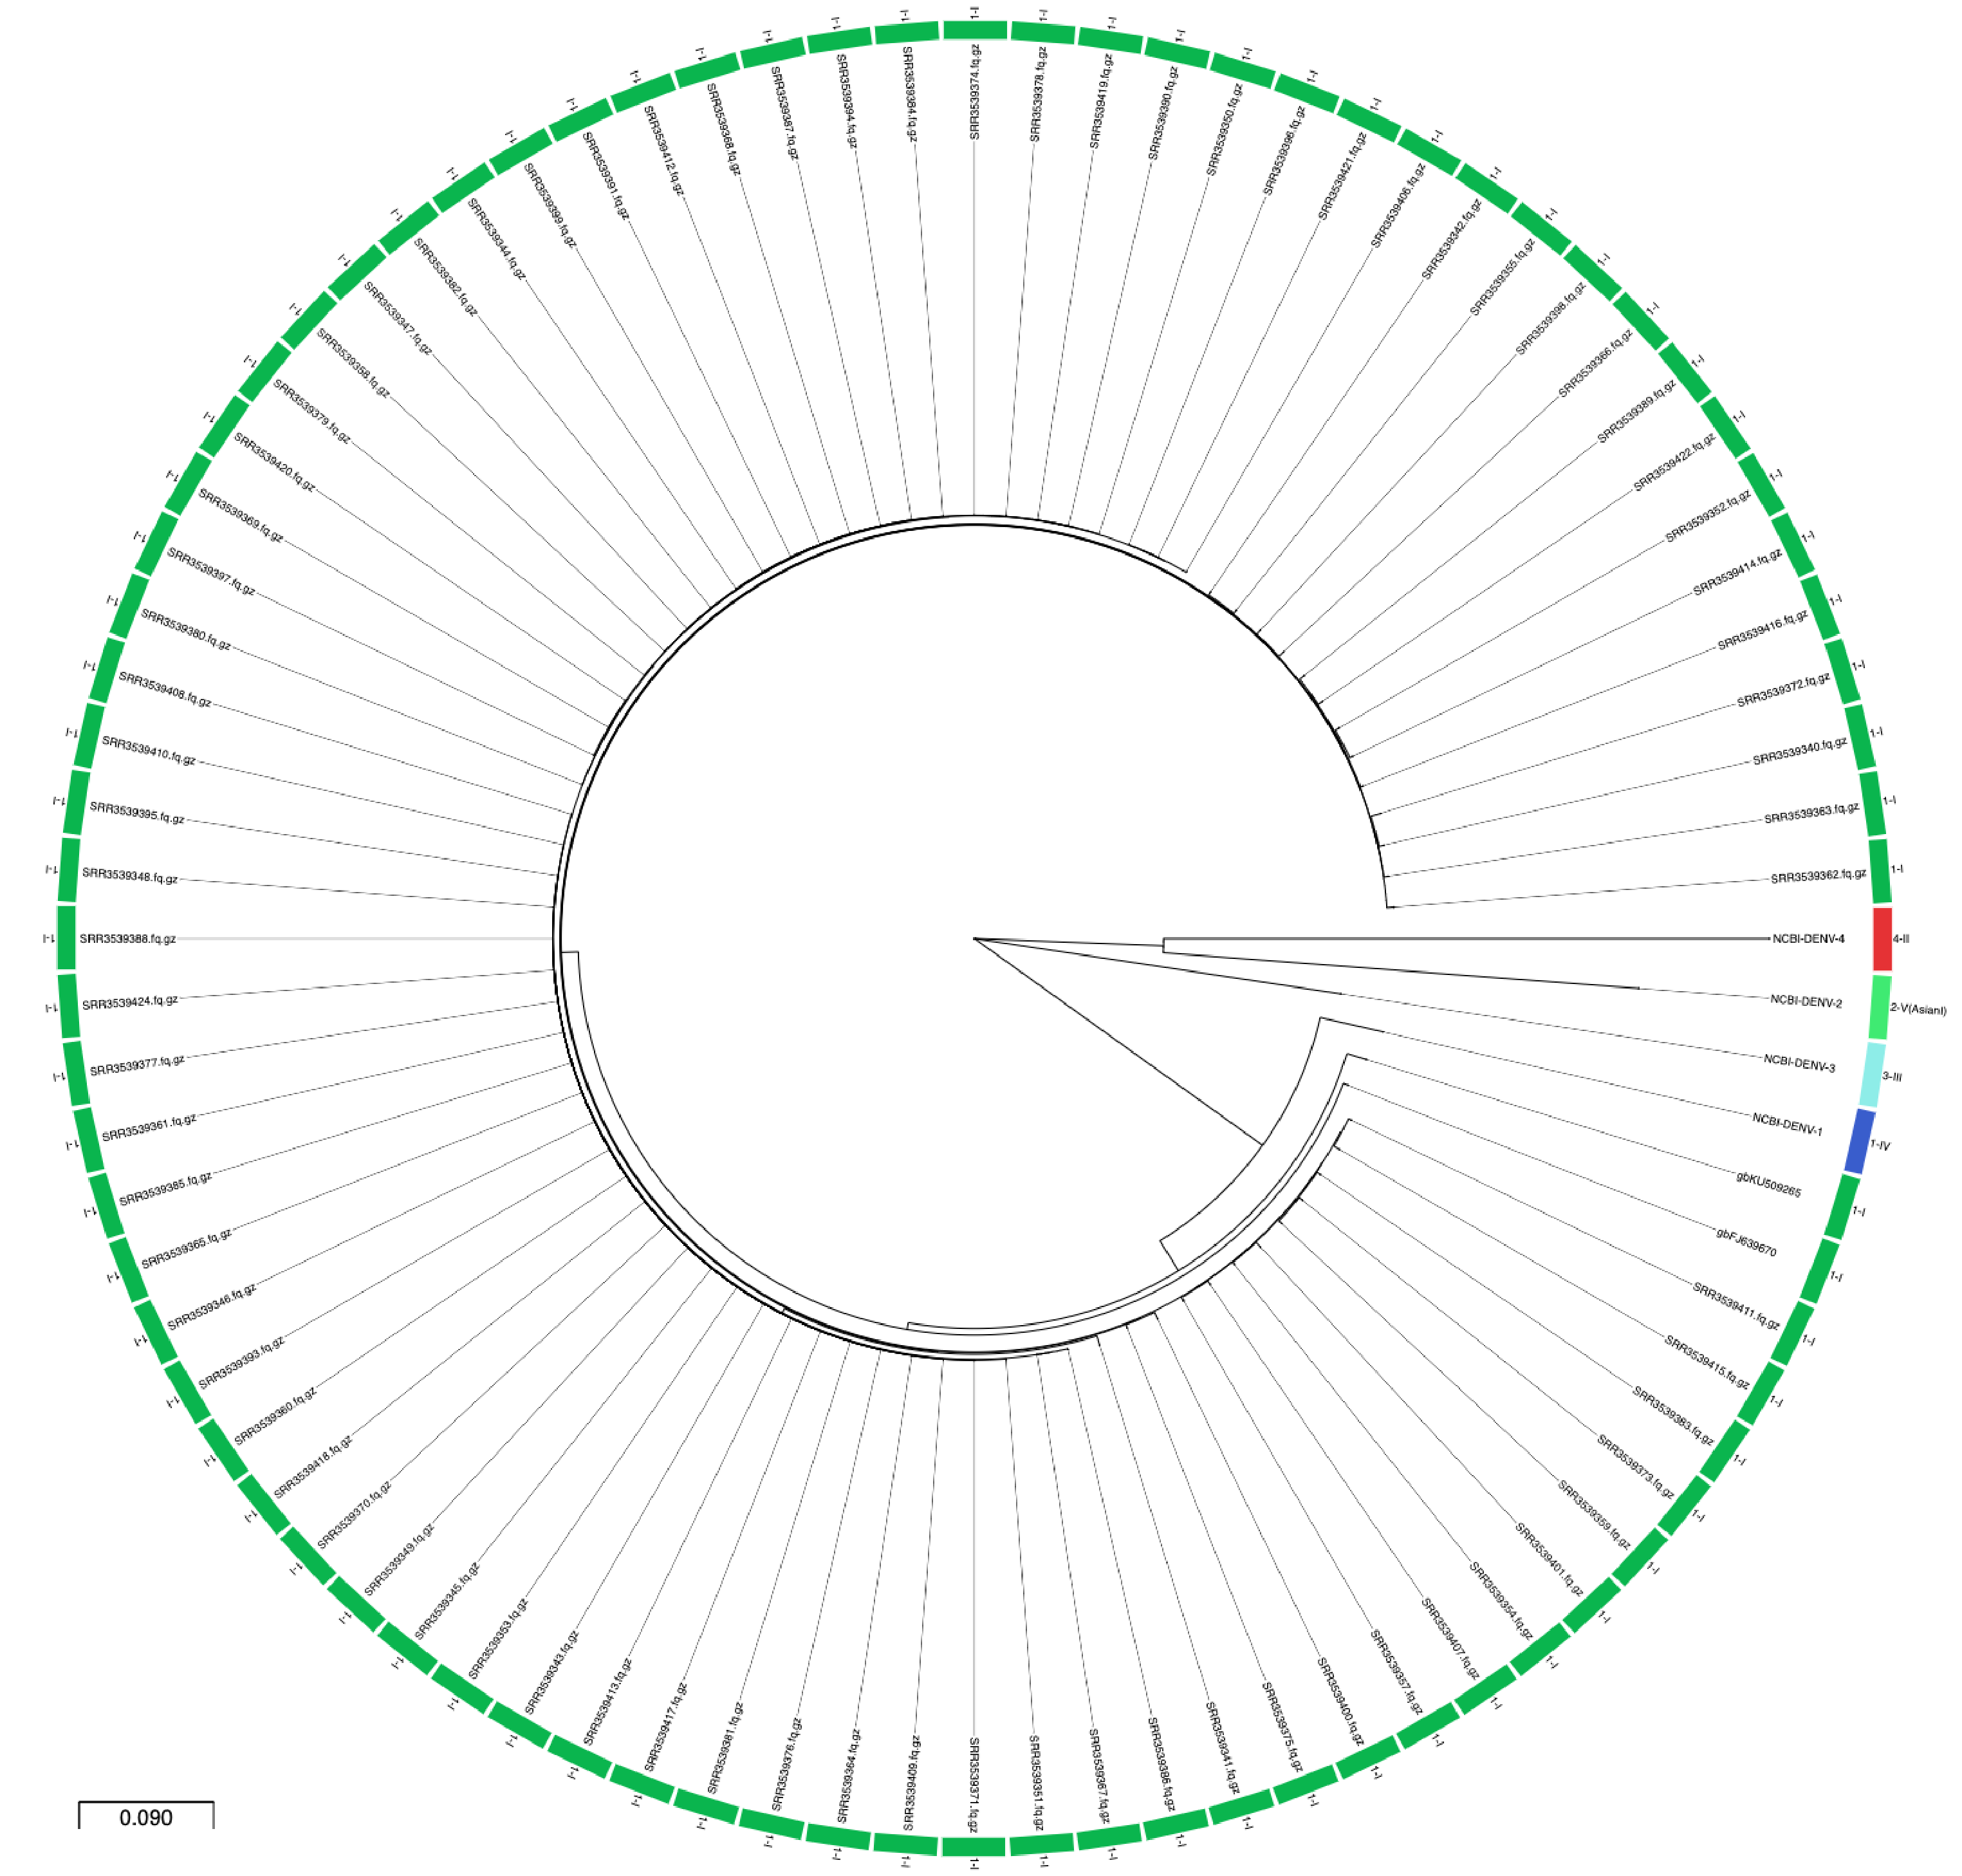
\includegraphics[width=\textwidth]{figures/chapter 4/Figure4.pdf}
\caption{Phylogenetic reconstruction of the single-end targeted metagenomic dataset. Maximum likelihood circular tree in the DEN-IM report for the 78 complete CDSs obtained with the targeted metagenomics dataset (n=78) and the NCBI DENV references for each serotype (NCBI-DENV-1: NC\_001477.1, NCBI-DENV-2: NC\_001474.2, NCBI-DENV-3: NC\_001475.2, NCBI-DENV-4: NC\_002640.1). All samples belong to serotype 1 genotype I. The scale represents average substitutions per site.}
\label{fig:chap4_figure4}
\end{figure*}

No samples failed the quality control block and the proportion of DENV reads ranged from 59\% (SRR3539343) to 96\% (SRR3539408) of the total processed reads (see Table \ref{}). Of the 78 samples, 53 (68\%) assembled a complete CDS sequence and in the remaining 25 (32\%) the complete CDS was obtained through mapping. All CDSs recovered, the respective closest reference genome in the typing database and NCBI’s references for each DENV serotype were aligned and a maximum likelihood phylogenetic tree was obtained (Figure \ref{fig:chap4_figure4}). All 78 samples belong to serotype 1 genotype I and, similarly to the previous dataset of 106 samples, there was detectable genetic diversity within the dataset (651 SNPs in 10808 nucleotides excluding reference sequences).


\subsubsection{The Non-DENV Arbovirus Dataset}

In order to evaluate DEN-IM’s specificity to DENV sequences, a third dataset of publicly available sequences of arbovirus other than DENV, both from amplicon and shotgun metagenomics, was analysed containing 45 CHIKV samples, 66 ZKV, and 21 YFV samples (see Table \ref{}). All 132 samples failed DEN-IM’s workflow, 16 due to not enough sequencing data remaining after quality trimming, and the remaining 116 due to very low estimated coverage of the DENV genome (less than 0.01x), as expected. 

\section{Conclusion}

We have successfully analysed two DENV datasets, one comprising 25 shotgun metagenomics sequencing samples and a second of 106 paired-end and 78 single-end targeted metagenomics samples. 

In the first dataset, we recovered 24 CDSs from 19 clinical samples, including a spiked sample and a positive control that were correctly serotyped and genotyped. Besides the negative control, 3 samples did not return typing information due to failing quality checks.

The proportion of DENV reads in the metagenomics samples was highly variable. This may reflect the viral load in patients in which DENV was detected by real-time RT-PCR. In the spiked sample, containing 4 distinct DENV serotypes, all four were correctly detected despite not being present in equal concentrations, highlighting the potential of the DEN-IM workflow to accurately detect and recover multiple DENV genomes from samples with DENV co-infection, even if the serotypes are present in low abundance. Indeed, recent studies from areas of high endemicity suggest that co-infection with multiple DENV serotypes may frequently occur \citep{marinho_meningitis_nodate, reddy_occurrence_2017} and the co-circulation of different DENV strains of the same serotype, but distinct genotypes, in these areas \citep{marinho_meningitis_nodate} raises the possibility of simultaneous infection with more than one genotype.

When analysing the 106 paired-end targeted metagenomics dataset, only 43 CDS samples were de novo assembled. For the remaining 63 samples, consensus sequences were obtained through mapping. In all samples DENV 3-III was correctly identified. Similar results were obtained for the 78 single-end samples where 53 CDS were de novo assembled, and 25 consensus sequences were obtained through mapping. All samples were identified as DENV-1 I. These two datasets demonstrate the success of DEN-IM’s two-pronged approach of combining assembler and mapping. DEN-IM’s specificity was shown when it found no false positive results when analysing a dataset containing arboviruses other than DENV. 

DEN-IM is built with modularity and containerisation as keystones, leveraging the parallelization of processes and guaranteeing reproducible analyses across platforms. The modular design allows for new modules to be easily added and tools that become outdated to be easily updated, ensuring DEN-IM’s sustainability. The software versions are also described in the Nextflow script and configuration files, and in the dockerfiles for each container, allowing the traceability of each step of data processing.

Being developed in Nextflow, DEN-IM runs on any UNIX-like system and provides out-of-the-box support for several job schedulers (e.g., PBS, SGE, SLURM) and integration with containerised software like Docker or Singularity. While it has been developed to be ready to use by non-experts, not requiring any software installation or parameter tuning, it can still be easily customised through the configuration files.

The interactive HTML reports (see \ref{}) provide an intuitive platform for data exploration, allowing the user to highlight specific samples, filter and re-order the data tables, and export the plots as needed.

Together with the workflow and software containers, a database containing 3858 complete DENV genomes for DENV sequence retrieval and a subset database with 161 curated DENV genomes for serotyping and genotyping are provided. While constructing these databases, the obstacles reported by Cuypers et al \citep{cuypers_time_2018} were apparent, namely the lack of formal definition of a DENV genotype and the lack of a standardised classification procedure that could assign sequences to a previously defined genotypic/sub-genotypic clade \citep{cuypers_time_2018}. Discrepancies between the phylogenetic relationship and the genotype assignment were frequent and, throughout this study, the classification of some strains within the ViPR database \citep{pickett_virus_2012} was updated. As suggested previously \citep{cuypers_time_2018}, further evaluation of the DENV classification will benefit future research and investigation into the population dynamics of this virus. Our typing approach was designed to use the currently accepted DENV classification. However, DEN-IM can be easily modified if a new DENV classification system is to be established in the future.

DEN-IM provides a user-friendly workflow that makes it possible to analyse short-read raw sequencing data from shotgun or targeted metagenomics for the presence, typing and phylogenetic analysis of DENV. The use of containerised workflows, together with shareable reports, will allow an easier comparison of results globally, promoting collaborations that can benefit the populations where DENV is endemic. The DEN-IM source code is freely available in the DEN-IM GitHub repository (\url{https://github.com/B-UMMI/DEN-IM}), which includes a wiki with full documentation and easy to follow instructions.

\section{Author Statements}

\subsection{Authors and contributions}

C.I.M., E.L., N.C., M.R., J.A.C. and J.W.A.R. designed the workflow. C.I.M implemented and optimised the workflow, created the Docker containers, and wrote the manuscript. M.P.M. implemented the DENV genotyping module in the workflow and D.N.S. contributed to the development of DEN-IM’s HTML report. E.L., A. T., and N.C. provided the shotgun metagenomics data used to test and validate the workflow and wrote the manuscript. A.T., N.C., M.R., J.A.C. and J.W.A.R. critically revised the article. All authors read, commented on, and approved the final manuscript.

\subsection{Conflict of interest}

The authors declare that they have no competing interests.

\subsection{Funding information}

C.I.M. was supported by the Fundação para a Ciência e Tecnologia (grant SFRH/BD/129483/2017). Erley Lizarazo received the Abel Tasman Talent Program grant from the UMCG, University of Groningen, Groningen, The Netherlands. This work was partly supported by the ONEIDA project (LISBOA-01-0145-FEDER-016417) co-funded by FEEI–Fundos Europeus Estruturais e de Investimento from Programa Operacional Regional Lisboa 2020 and by national funds from FCT–Fundação para a Ciência e a Tecnologia and by UID/BIM/50005/2019, project funded by Fundação para a Ciência e a Tecnologia (FCT)/ Ministério da Ciência, Tecnologia e Ensino Superior (MCTES) through Fundos do Orçamento de Estado.

\subsection{Ethical approval}

This study followed international standards for the ethical conduct of research involving human subjects. Data and sample collection was carried out within the DENVEN and IDAMS (International Research Consortium on Dengue Risk Assessment, Management and Surveillance) projects. The study was approved by the Ethics Review Committee of the Biomedical Research Institute, Carabobo University (Aval Bioetico #CBIIB(UC)-014 and CBIIB-(UC)-2013-1), Maracay, Venezuela; the Ethics, Bioethics and Biodiversity Committee (CEBioBio) of the National Foundation for Science, Technology and Innovation (FONACIT) of the Ministry of Science, Technology and Innovation, Caracas, Venezuela; the regional Health authorities of Aragua state (CORPOSALUD Aragua) and Carabobo State (INSALUD); and by the Ethics Committee of the Medical Faculty of Heidelberg University and the Oxford University Tropical Research Ethics Committee.

\subsection{Consent for publication}

All individuals, or a parent or legal guardian if under 16 years of age, whose sample and data were collected have given consent to participate in the study.

\subsection{Acknowledgements}

The authors would like to thank Tiago F. Jesus and Bruno Ribeiro-Gonçalves for their invaluable help with the Nextflow implementation. We would also like to thank Erwin C. Raangs from the UMCG for his assistance in the sequencing of the shotgun metagenomics dataset. Additionally, the authors thank Lize Cuypers, Krystof Theys, Pieter Libin and Gilberto Santiago for their discussions on DENV nomenclature and classification. This work was done in collaboration with the ESCMID Study Group on Molecular and Genomic Diagnostics (ESGMD), Basel, Switzerland.

\section{Data Bibliography}
\begin{itemize}
    \item Catarina Inês Mendes. DEN-IM supplemental material and tables are deposited at Figshare with DOI 10.6084/m9.figshare.9963812 (https://doi.org/10.6084/m9.figshare.9963812.v3).
    \item Catarina Inês Mendes. DEN-IM reports for the analysed datasets tables are deposited at Figshare with DOI 0.6084/m9.figshare.9318851 (https://doi.org/10.6084/m9.figshare.9318851).
    \item Catarina Inês Mendes. Phylogeny inference trees for the dengue virus typing database are deposited at Figshare with DOI 10.6084/m9.figshare.9331826 (https://doi.org/10.6084/m9.figshare.9331826).
    \item Catarina Inês Mendes. Code for the DEN-IM workflow (https://github.com/B-UMMI/DEN-IM).
\end{itemize}

\section{Supplementary Material}

\subsection{Dengue virus reference databases} \label{chap4_sup_database}

We have compiled a database of 3858 complete DENV genomes obtained from the NIAID Virus Pathogen Database and Analysis Resource (ViPR) in October 2019 \citep{pickett_virus_2012} (\url{http://www.viprbrc.org/}).The sequences were distributed unevenly throughout the four DENV serotypes, with DENV-1 being the most represented with 1636 sequences (42.72\%), followed by DENV-2 with 1067 sequences (27.86\%), DENV-3 with 807 sequences (21.07\%), and DENV-4 with 320 sequences (8.36\%). The selection criteria for the search were as follows: a) complete genome sequence only, b) human or mosquito host, c) collection year (1950-2018). Data available from all countries was included and duplicated sequences were removed and only the sequences with sub-type data were kept. A representative of DENV serotype 1 genotype III was introduced (EF457905, recovered from monkey) as no representatives were available with the search criteria used. This genotype is sylvatic and considered extinct \citep{villabona-arenas_worldwide_2013, vasilakis_history_2008}. Additionally, any sample with IUPAC codes in the sequence provided were excluded. 

In order to recover the maximum number of DENV reads from the input HTS data in the first mapping step (Figure \ref{fig:chap2_figure1}), we maintained the database with the 3858 complete DENV genomes to retain as much diversity as possible. This database is referred as DENV mapping database and is available on GitHub at \url{https://github.com/B-UMMI/DEN-IM/blob/master/ref/DENV_MAPPING_V3.fasta}. 

For typing purposes, overly similar sequences in the collection were removed from the database by clustering the sequences in each serotype at 98\% nucleotide similarity with CD-HIT \citep{li_cd-hit_2006}, leaving 161 representative sequences of all described DENV serotypes and genotypes, with 46 DENV-1 sequences (Table), 63 DENV-2 (Table), 25 DENV-3 (Tables) and 27 DENV-4 (Table). This database is referred as DENV typing database and is available on GitHub at \url{https://github.com/B-UMMI/DEN-IM/blob/master/ref/DENV_TYPING_V3.fasta}. This step is necessary to speed up the classification step for genotyping.

Phylogenetic analysis of typing collection was performed by aligning the full reference genomes with MAFFT \citep{nakamura_parallelization_2018}, in auto mode and with automatic sequence orientation adjustment. A phylogenetic tree was inferred with RAxML (version 8.12.11) \citep{stamatakis_raxml_2014} using the GTR-$\Gamma$ substitution model and 500 times bootstrap. Additionally, the same analysis was performed with the envelope protein (E) only, as this region has been used traditionally for sero- and genotyping \citep{rico-hesse_molecular_1990, rico-hesse_microevolution_2003, lanciotti_rapid_1992, lanciotti_molecular_1997, klungthong_molecular_2004, zhang_clade_2005, zhang_structure_2006}, and continues to be the standard in many laboratories for genotyping. The resulting trees are available as supplemental material (Figures to ) and on Figshare (\url{https://10.6084/m9.figshare.9331826}).

The sequence JF459993 from the DENV-1 collection, as of April 2019, was annotated in ViPR as belonging to genotype IV, but in our analysis, it clustered within genotype I clade (Figure ). The classification of DENV-1 I was also obtained from GenomeDetective Dengue Subtyping Tool (\url{https://www.genomedetective.com/app/typingtool/dengue/}), so we proceeded to alter the annotation of this particular sample (Table). 
In order to harmonise dengue nomenclature, the system uses Roman-numeric labels to identify the genotype, with the exception of Serotype 2 (Table), which used both Roman-numeric and geographic origin due to the widespread adoption of the latter.

\subsection{Workflow parameters} \label{chap4_sup_workflow_params}

The short-read data is passed as input through the “--fastq” parameter, that by default is set to match all files in the “fastq” folder that match the pattern “*\_R{1,2}*”. Both paired and single-end sequencing data can be passed through with the “--fastq” parameter, as defined by the pattern used. 

In the process to verify the integrity of the short-read raw sequencing data, the integrity of the input files is assessed by attempting to decompress and read the files. An estimation of the depth of coverage is also performed. By default, the input size ("–-genomeSize") is set to 0.012 Mb and the minimum coverage depth ("–-minCoverage") is set to 10. If any input file is found to be corrupt, its progression in the workflow is aborted.

In the FastQC and Trimmomatic module, FastQC (https://www.bioinformatics.babraham.ac.uk/projects/fastqc/) is run with the parameters "–extract –nogroup –format fastq". FastQC will inform Trimmomatic \citep{bolger_trimmomatic_2014} on how many bases to trim from the 3’and 5’ ends of the raw reads. By default, Trimmomatic uses the default set of Illumina adapters provided with the workflow but this behaviour can be overwritten with the "–-adapters" parameter. The additional Trimmomatic parameters "-–trimSlidingWindow", "–-trimLeading", "–-trimTrailing" and "–-trimMinLength"can all be set to different values.

The removal of low complexity sequences is done with PrinSeq \citep{schmieder_quality_2011} using a custom parameter ("–pattern"), which by default is set to the value "A 50\%; T 50\%; N 50\%", removing sequences whose content is at least half composed of a polymeric sequence (A, T or N).

To retrieve the reads that map to the DENV reference database, Bowtie2 \citep{langmead_fast_2012} is run with default parameters with the DENV mapping database as a reference. For paired-end data, the reads and their mates that map to the reference are retrieved with "samtools view -buh -F 12" and "samtools fastq" commands. In single-end reads, all mapped reads are retrieved with "samtools view -buh -F 4" and "samtools fastq". The DENV mapping database can be altered with the "–-reference" parameter, or alternatively, a Bowtie2 index can be provided with the "–-index" parameter. This allows for the workflow to work with other databases obtained through public and owned DENV genomes. The coverage estimation step is performed on the retrieved DENV reads with the same parameters are the first estimation ("–-genomeSize=0.012" and "–-minCoverage=10").

In the assembly process, the retrieved DENV reads are firstly assembled with SPAdes Genome Assembler \citep{bankevich_spades_2012} with the options "–careful –only-assembler –cov-cutoff". The coverage cut-off if dictated by the "–-spadesMinCoverage" and "–-spadesMinKmerCoverage" parameters, set to 2 by default. If the assembly with SPAdes fails to produce a contig equal or greater than the value defined in the "–minimumContigSize" parameter (default of 10000), the data is re-assembled with the MEGAHIT assembler \citep{li_megahit_2015} with default parameters. By default, the k-mers to be used in the assembly in both tools ("–spadesKmers" and "–megahitKmers") are automatically determined depending on the read size. If the maximum read length is equal or greater than 175 nucleotides, the assembly is done with the k-mers "55, 77, 99, 113, 127", otherwise the k-mers "21, 33, 55, 67, 77" are used.

To correct the assemblies produced, the Pilon tool \citep{walker_pilon_2014} is run after mapping the QC’ed reads back to the assembly with Bowtie2 and "samtools sort". This process also verifies the coverage and the number of contigs produced in the assembly. The behaviour can be altered with the parameters "–minAssemblyCoverage", "–AMaxContigs" and "–genomeSize", set to "auto", 1000 and 0.01 Mb by default. The first parameter, when set to ’auto’, the minimum assembly coverage for each contig required is set to the 1/3 of the assembly mean coverage or to a minimum of 10x. The ratio of contig number per genome MB is calculated based on the genome size estimation for the samples.
The contigs larger than the value defined in the "–size" parameter (default of 10000 nucleotides) are considered to be complete CDSs and follow the rest to the workflow independently. If no complete CDS is recovered, the QC’ed read data is passed to the mapping to module that does the DENV typing database and consensus generation. 

The serotyping and genotyping are performed with the Seq\_Typing tool \citep{machado_epidemiological_2017} with the command "seq\_typing.py assembly" or "seq\_typing.py reads", using as reference the provided curated DENV typing database. It is possible to retrieve the genomes of the closest references and include them in the downstream analysis by changing the "–get\_reference" option to "true". By default, this is not included in the analysis.

The CDSs, and the reference sequences if requested, are aligned with the MAFFT tool \citep{nakamura_parallelization_2018} with the options "–adjustdirection –auto". By default, four representative sequences for each DENV serotype (1 to 4) from NCBI is also included in the alignment. This option can be turned off by changing the value of “--includeNCBI” to "false". If the number of sequences in the alignment is less than 4 these are automatically added. 

A maximum likelihood phylogenetic tree is obtained with the RaXML tool \citep{stamatakis_raxml_2014} with the options "-p 12345 -f -a". Additionally, and by default, the substitution model ("–substitutionModel") is set to "GTRGAMMA", the bootstrap is set to 500 ("–bootstrap") and the seed to "12345" ("–seedNumber").

\subsection{Shotgun Metagenomics Sequencing Data} \label{chap4_sup_data}

Samples of plasma (n=9) and serum samples (n=13) from confirmed dengue symptomatic patients were collected in Venezuela between 2010-2015 (Table S2) (see Availability of supporting materials). DENV positivity was confirmed by either RT-qPCR \citep{santiago_analytical_2013} or nested RT-PCR \citep{lanciotti_rapid_1992}. 

As a positive control sample, the supernatant of a viral culture containing DENV-2 strain 16681 was used. The negative control sample consisted of DNA- and RNA-free water (Sigma-Aldrich, St. Louis, MO, USA). 

A spiked sample was produced consisting of a mixture of four 5 µl of cDNA isolated from clinical samples including all DENV serotypes (DENV-1 to -4). The viral cDNA for these samples was not in equal concentration and the viral copy number in the clinical samples was assessed by RT-PCR \citep{lanciotti_rapid_1992}. The results were as follow: DENV-2 with 1070000 copies/µl, DENV-1 with 117830 copies/µl, DENV-3 with 44300 copies/µl and DENV-4 with 6600 copies/µl.

The cDNA libraries were generated using either the NEBNext® RNA First and Second strand modules and the Nextera XT DNA library preparation kit (NXT), or the TruSeq RNA V2 library preparation kit (TS). The libraries were sequenced in MiSeq and NextSeq instruments using 300-cycles v2 paired-end cartridges.

The DEN-IM workflow was executed with the raw sequencing data using the default parameters and resources in an HPC cluster with 300 Cores/600 Threads of Processing Power and 3 TB RAM divided through 15 computational nodes, 9 with 254 GB Ram and 6 with 126GB RAM.

\subsection{Amplicon Sequencing Data} \label{chap4_sup_amplicon}

The accession numbers for the 106 DENV-3 paired-end amplicon sequencing paired-end short-read datasets are available under BioProject PRJNA394021. The accession numbers for the 78 DENV-1 amplicon sequencing single-end short-read datasets are available under BioProject PRJNA321963. The Run Accession IDs for both sets were obtained with NCBI’s RunSelector and the raw data was downloaded with the GetSeqENA tool (https://github.com/B-UMMI/getSeqENA).

The DEN-IM workflow was executed with the raw sequencing data with default parameters and resources in the same HPC cluster as the shotgun metagenomics dataset.

\subsection{Non-DENV Arbovirus Data} \label{chap4_sup_non_denv}

The accession numbers for the 132 samples, belonging to zika virus (ZKV), chikungunya virus (CHIKV) and yellow fever virus (YFV) amplicon and metagenomic datasets are available as supplemental material (Table S4). As with the amplicon sequencing dataset, the list of Run Accession IDs was obtained with NCBI’s RunSelector and the raw data was downloaded with the GetSeqENA tool (https://github.com/B-UMMI/getSeqENA). 

The DEN-IM workflow was executed with default parameters and resources in the same HPC cluster as the amplicon and shotgun metagenomics datasets.

\subsection{Supplemental Tables} \label{chap4_sup_tables}

\subsection{Supplemental Figures} \label{chap4_sup_figures}

\begin{figure*}[h!]
\centering
\includegraphics[width=\textwidth]{figures/chapter 4/}
\caption{DEN-IM report tables. a) DEN-IM's quality control report containing information of the number of base-pairs and the number of reads for the analysed samples, the estimated coverage depth before and after mapping, and the percentage of reads in the input data that were trimmed. b) DEN-IM's typing report for 24 CDSs recovered from the metagenomic dataset. The ID contains the CDS contig name, the typing result for serotype-genotype, the values for identity and coverage, and the GenBank ID of the closest reference in the Typing Database containing 161 complete DENV genomes.}
\label{fig:chap4_figure_sup1}
\end{figure*}